\documentclass{article}
\usepackage{import}
\usepackage[ruled]{algorithm2e}
\usepackage[shortlabels]{enumitem}
\usepackage{hyperref}
\usepackage{minted}
\usepackage{subcaption}

\hypersetup{
    colorlinks=true,
    linkcolor=blue,
    filecolor=magenta,      
    urlcolor=cyan,
    pdftitle={Overleaf Example},
    pdfpagemode=FullScreen,
    }
\subimport*{}{macro}

\setlength\parindent{0px}

\begin{document}
\setcounter{problem}{0}
\title{Homework \#3}
\author{
    \normalsize{AA 597: Networked Dynamics Systems}\\
    \normalsize{Prof. Mehran Mesbahi}\\
    \normalsize{Due: Feb 2, 2024 11:59pm}\\
    \normalsize{Soowhan Yi}
}
\date{{}}
\maketitle

All the codes are available at the end of the documents or here.
\url{https://github.com/SoowhanYi94/ME597}
\begin{problem}
    How would one extend Exercise 3.6 to n particles in three dimensions?

    First, random graphs with n nodes were created with m edges, and their positions were initialized randomly.  Then calculate inputs using $u_i = -(L(D)_{ij} * (x_j - x_i) + L(D)_{ij}( v_j - v_i)) $
    \begin{minted}{python3}
def get_input(x, G):
    k_p = 1
    k_v = 1
    u = np.zeros(len(x)//2)
    L_D = list(nx.directed_laplacian_matrix(G))
    for i in G.nodes():
        for j in G.neighbors(i):
            u[i] += -(k_p * L_D[i][j] * (x[j]- x[i] ) 
            + k_v *L_D[i][j]* (x[len(x)//2 + j] - x[len(x)//2 + i] ))
    return u
    \end{minted}
    In this code, x is a list of values of position and velocity in a direction. i.e. $x = [p_1, p_2 \cdots p_n, v_1, v_2 \cdots, v_n]$. It can be used for x, y, and z direction. 
    \begin{minted}{python3}
def get_xdot(x, t, G):
    num = len(x)
    A = np.array([[0, 1], [0, 0]])
    B = np.array([0, 1])
    Kronecker_A = np.kron(A, np.eye(num//2))
    u = get_input(x, G)
    dxdt = np.matmul(Kronecker_A, x) + np.kron(B, u)
    return dxdt 
    \end{minted}
    \begin{align*}
        \frac{d}{dt} 
        \begin{bmatrix*}
            p_i(t)\\
            v_i(t)  
        \end{bmatrix*}
        = \begin{bmatrix*}
            0 & 1\\
            0 & 0 
        \end{bmatrix*}
        \begin{bmatrix*}
            p_i(t)\\
            v_i(t)  
        \end{bmatrix*}
        + 
        \begin{bmatrix*}
            0\\
            1
        \end{bmatrix*} u_i(t)
    \end{align*}
    Through using Kronecker product, the above equation can be expressed as such $ A \otimes I_{a} x + B \otimes u $, where $x = [p_1, p_2 \cdots p_n, v_1, v_2 \cdots, v_n]$ and $I_{a}$ is identity matrix with a (number of nodes) rows. . Simulation result is shown below. 
    \newpage
    \begin{figure*}[!h]
        \centering
        \begin{subfigure}{0.35\textwidth}
            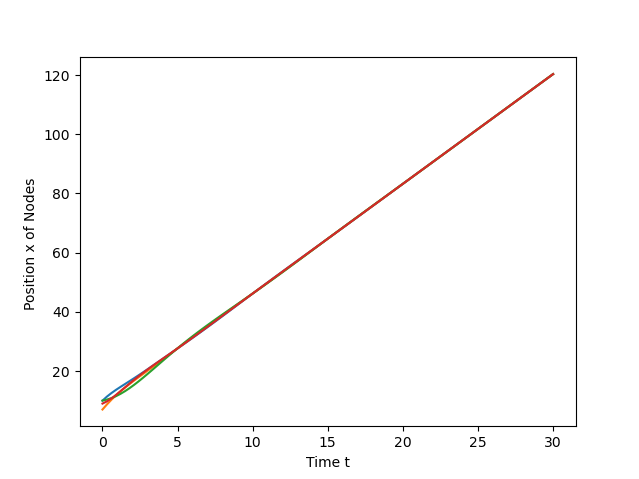
\includegraphics[width=\textwidth]{./img/p1_1.png}
            \caption{x direction position trajectory}
        \end{subfigure}
        \begin{subfigure}{0.35\textwidth}
            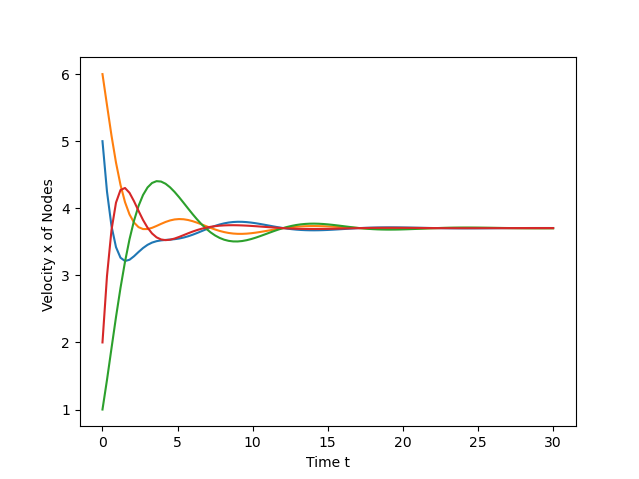
\includegraphics[width=\textwidth]{./img/p1_2.png}
            \caption{x direction velocity trajectory}
        \end{subfigure}
        \begin{subfigure}{0.35\textwidth}
            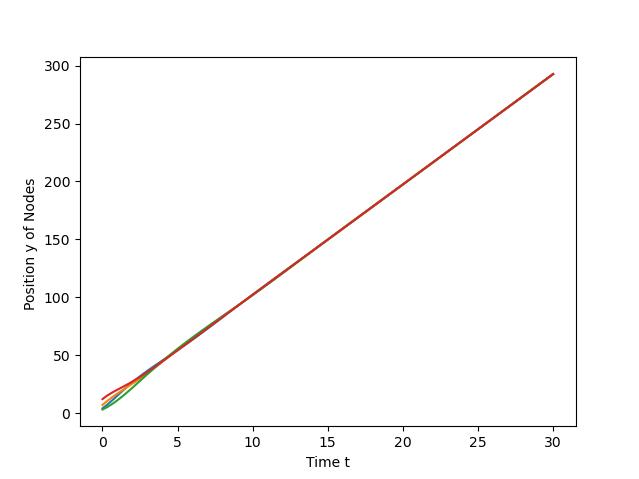
\includegraphics[width=\textwidth]{./img/p1_3.png}
            \caption{y direction position trajectory}
        \end{subfigure}
        \begin{subfigure}{0.35\textwidth}
            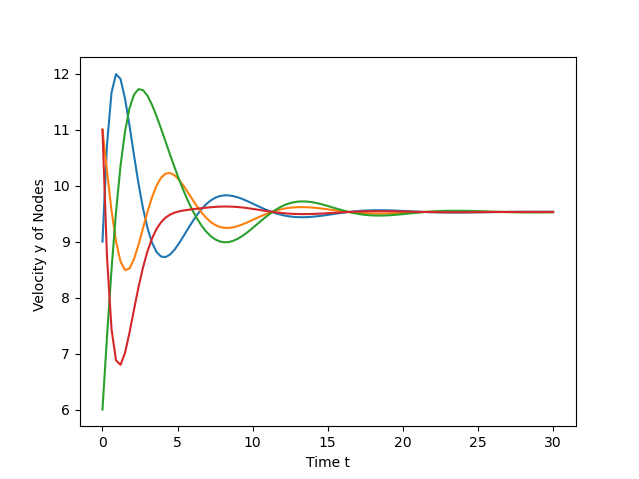
\includegraphics[width=\textwidth]{./img/p1_4.png}
            \caption{y direction velocity trajectory}
        \end{subfigure}
        \begin{subfigure}{0.35\textwidth}
            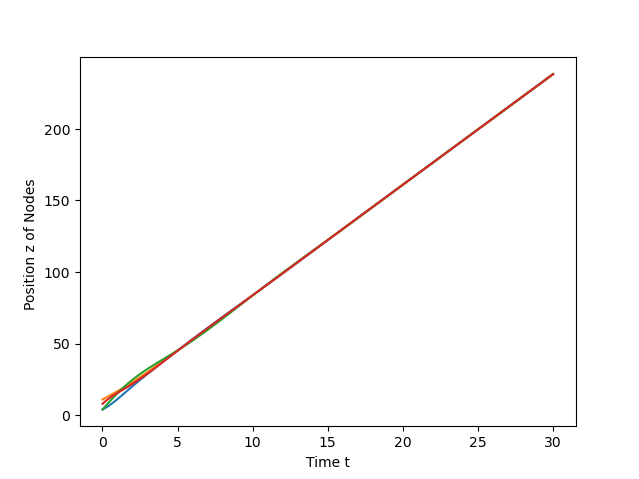
\includegraphics[width=\textwidth]{./img/p1_5.png}
            \caption{z direction position trajectory}
        \end{subfigure}
        \begin{subfigure}{0.35\textwidth}
            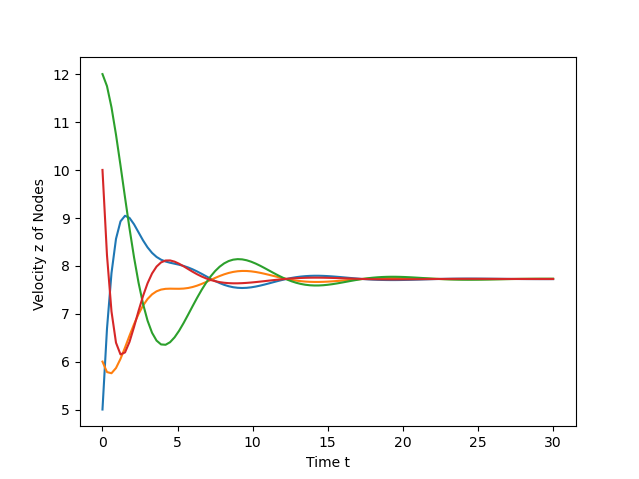
\includegraphics[width=\textwidth]{./img/p1_6.png}
            \caption{z direction velocity trajectory}
        \end{subfigure}
        \begin{subfigure}{0.35\textwidth}
            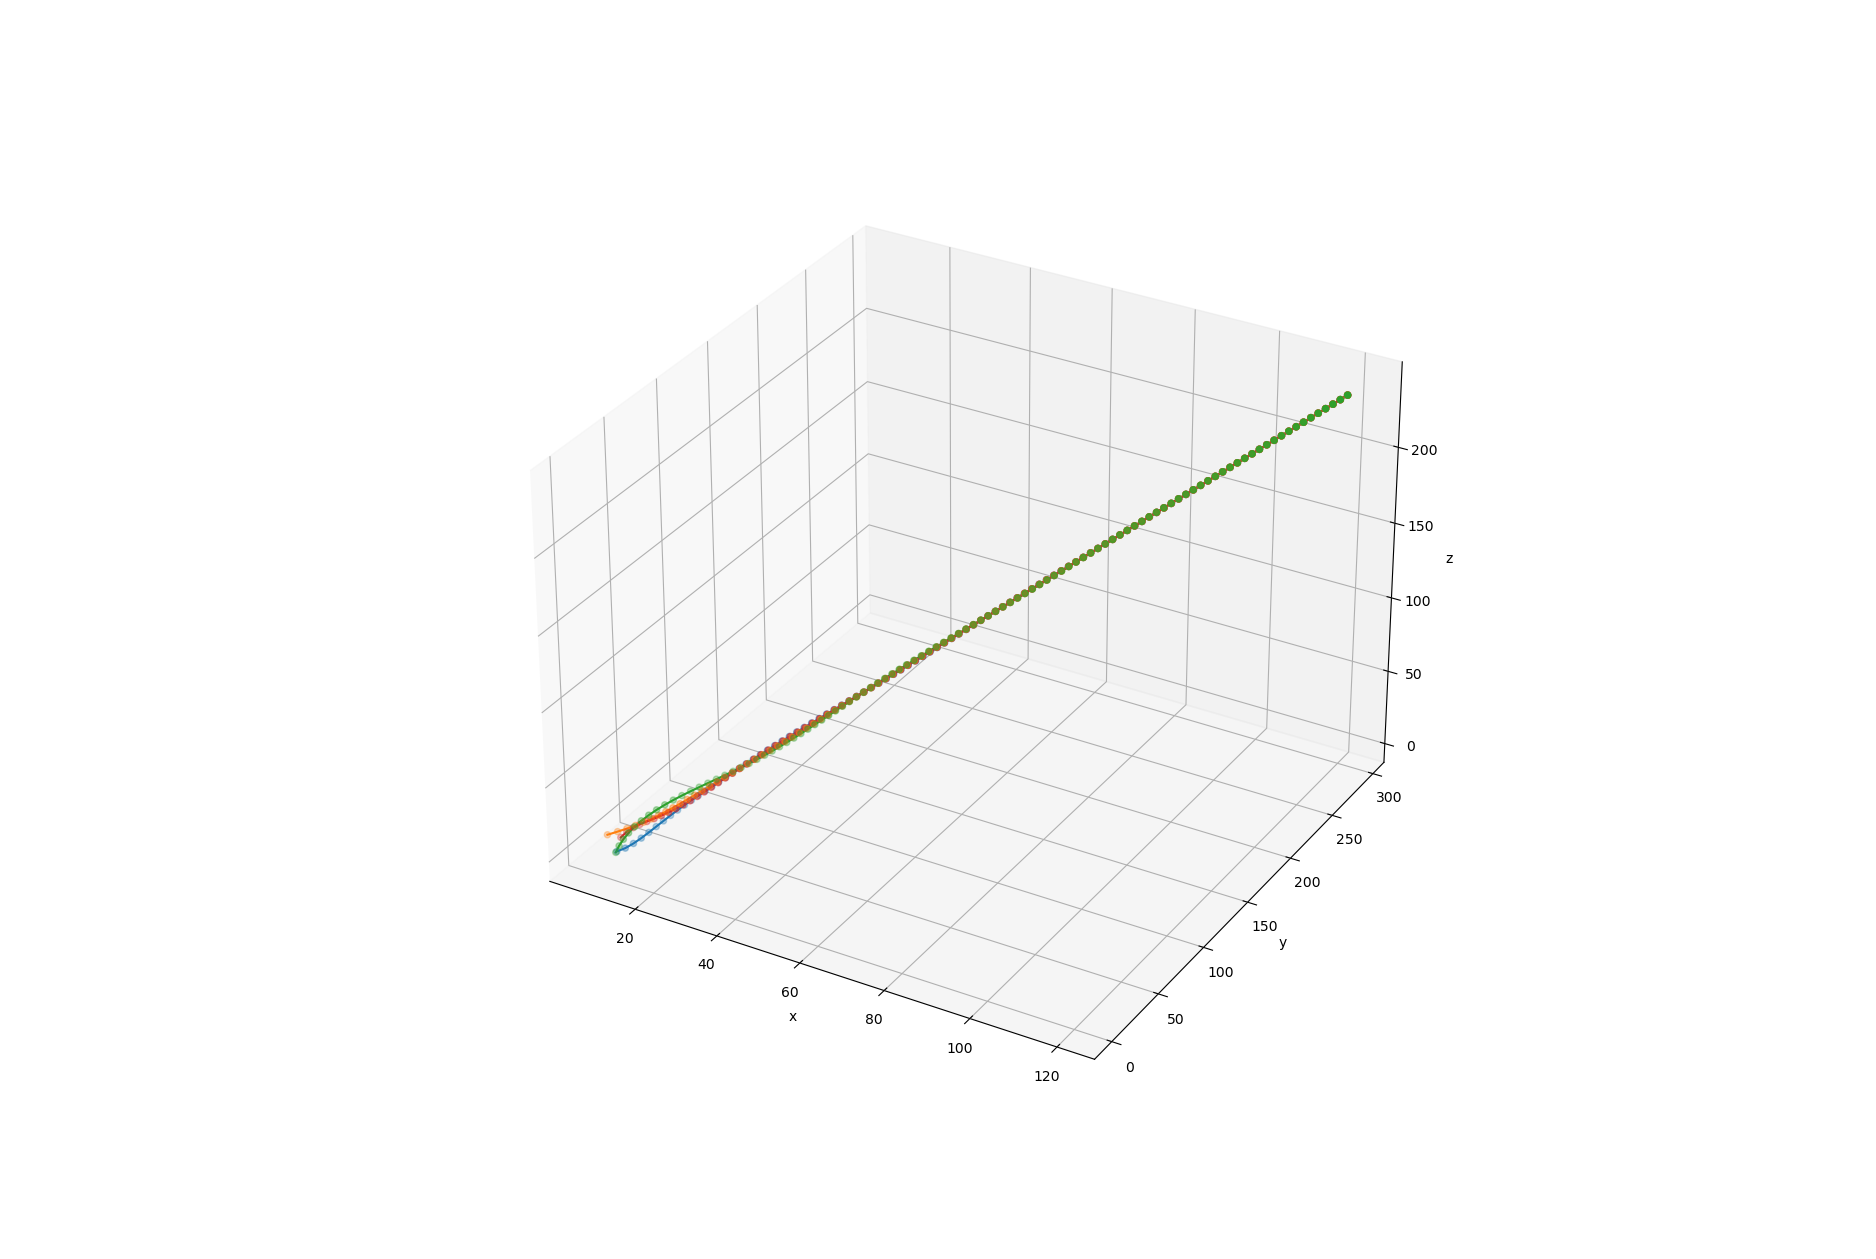
\includegraphics[width=\textwidth]{./img/p1_augmented.png}
            \caption{3 d position trajectory}
        \end{subfigure}
    
    \end{figure*}
    Here, I used 4 nodes for simplicity.
    If we were to augment the x,y, and z direction in to the poistion, we can use \\$x =  [p_{x_1}, p_{x_2} \cdots p_{x_n},p_{y_1}, p_{y_2} \cdots p_{y_n}, p_{z_1}, p_{z_2} \cdots p_{z_n}, v_{x_1}, v_{x_2} \cdots, v_{z_n}]$, and change equation using Kronecker product, accordingly. 
    % \begin{align*}
    %     A \otimes I_{3a} x + B \otimes I_{3b} u 
    % \end{align*}
\end{problem}
\begin{problem}
    \begin{align*}
        \dot{x}_i(t) = \sum_{j \in N(i)} (x_j(t) - x_i(t)), \space i = 1, \cdots , n
    \end{align*}
    Consider vertex i in the context of the agreement protocol(3.1). Suppose that vertex i (the rebel) decides not to abide by the agreement protocol, and instead fixes its state to a constant value. Show that all vertices converge to the state of the rebel vertex when the graph is connected.
    
    1. Prove that the graph contains rooted out branching
    
    Since the graph is connected, the rebel vertex must have rooted out branch.

    2. Jordan decomposition
    
    Since the rebel vertex, i, is not affected by the other nodes, the agreement protocol matrix  or the in-degree laplacian matrix would have row of zeros in ith row. e.i $x_{rebel} = x_i$ and $\dot x_i = [0 0 0 0 \cdots 0] x $. Using Jordan decomposition of $L(D)$, we know that this row of zeros would lead to $\lambda_1 = 0$, from proposition 3.11 and theorem 3.12 of the textbook. Using the proposition and the theorem, we now know that left eigenvector $(q_1)$ and the right eigenvector $(p_1)$ leads to agreement, $\lim_{t\rightarrow \infty} x(t) = p_1 q_1 x(0)$. Because the in-degree laplacian matrix contains row of zeros at ith row, $q_1 = [0 0 0 \cdots 1 0 0 \cdots 0]$ is also a left eigen vector associated with zero eigenvalue.  Also we can choose vector of ones for $p_1$ because it belongs to span of 1. Then $\lim_{t\rightarrow \infty} x(t) = p_1 q_1 x(0) = x_i(0)$. Therefore it would converge to state of the rebel vertex.    
\end{problem}
\begin{problem}
    Consider the system
    \begin{align*}
        \dot{\theta}_i(t) = \omega_i + \sum_{j \in N(i)} sin(\theta_j(t) - \theta_i(t)), \text{  for } i = 1, 2, 3, \cdots, n
    \end{align*}
    which resembles the agreement protocol with the linear term $x_j - x_i$ replaced by the nonlinear term $sin(\theta_j(t) - \theta_i(t))$. For $\omega_i = 0$, simulate (4.35) for $n = 5$ and various connected graphs on five nodes. Do the trajectories of (4.35) always converge for any initialization? How about for $\omega_i \neq 0$? (This is a "simulation-inspired question" so it is okay to conjecture!) 

    \begin{minted}{python3}
def get_thetadot(theta, t, G, omega):
    D = nx.incidence_matrix(G).toarray()
    dxdt = omega + np.matmul(D,np.matmul(D.T, np.sin(theta)))
    return dxdt 
    \end{minted}
    With above code, implements the Kuramoto model and it shows that the trajectories of headings do not necessarily converge to one value. Only the complete graph guranteed convergence, at least for my multiple iterations. But, through multiple iterations, some graphs do converge with random initialization. The reason for this convergence is that $|\theta_j(t) - \theta_i (t)| \leq \frac{\pi}{2}$. If $|\theta_j(t) - \theta_i (t)| \geq \frac{\pi}{2}$, then  $sin(\theta_j(t) - \theta_i (t))$ term would become negative and cause the nodes to push away from convergence. But, in case of complete graph, the nature of laplacian matrix(symetric and positive semi definite) of it leads to the convergence to average of their headings. 
    \begin{figure*}[!h]
        \centering
        \begin{subfigure}{0.35\textwidth}
            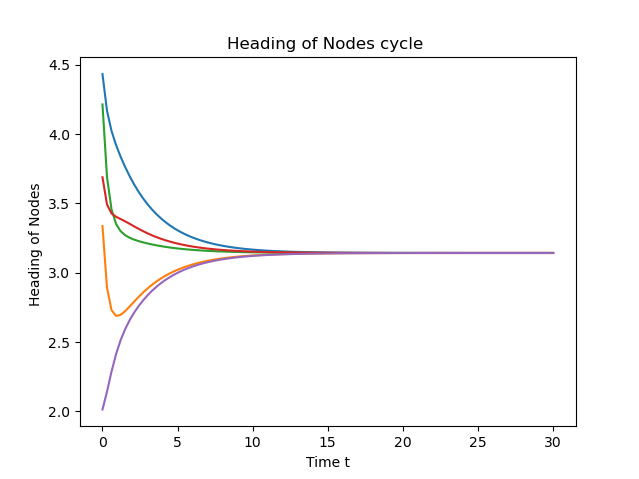
\includegraphics[width=\textwidth]{./img/p3_cycle0.png}
            \caption{Theta convergence of cycle graph }
        \end{subfigure}
        \begin{subfigure}{0.35\textwidth}
            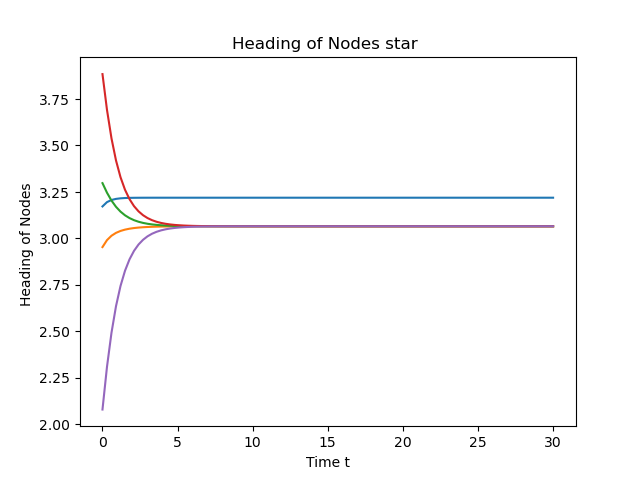
\includegraphics[width=\textwidth]{./img/p3_star0.png}
            \caption{Theta convergence of star graph }
        \end{subfigure}
        \begin{subfigure}{0.35\textwidth}
            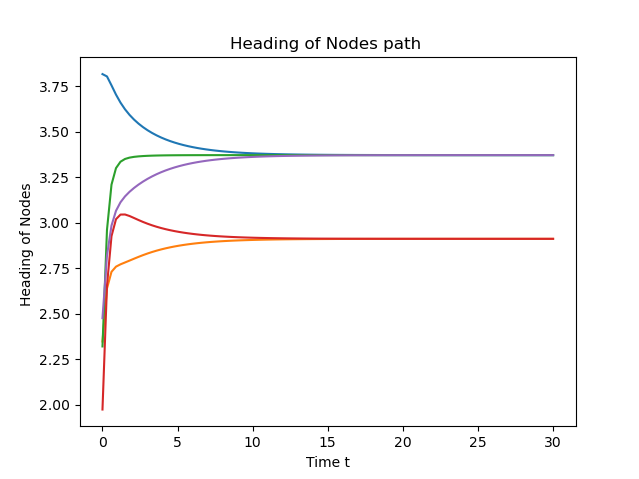
\includegraphics[width=\textwidth]{./img/p3_path0.png}
            \caption{Theta convergence of path graph }
        \end{subfigure}
        \begin{subfigure}{0.35\textwidth}
            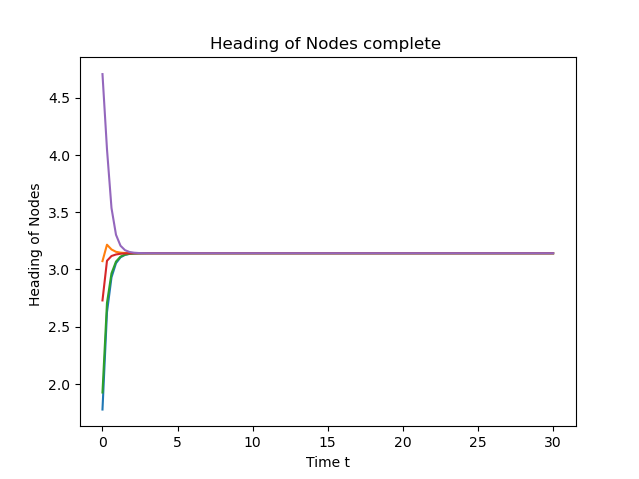
\includegraphics[width=\textwidth]{./img/p3_complete0.png}
            \caption{Theta convergence of complete graph }
        \end{subfigure}
    \end{figure*} 
    \newpage
    As you can see from above graphs, only graphs that converged are cycle and complete graph. Now lets look at the case where $\omega_i = 1$ and $\omega = [1 0 1 0 0]$,respectively  (it was randomly chosen by me)
    \newpage
    \begin{figure*}[!h]
        \centering
        \begin{subfigure}{0.35\textwidth}
            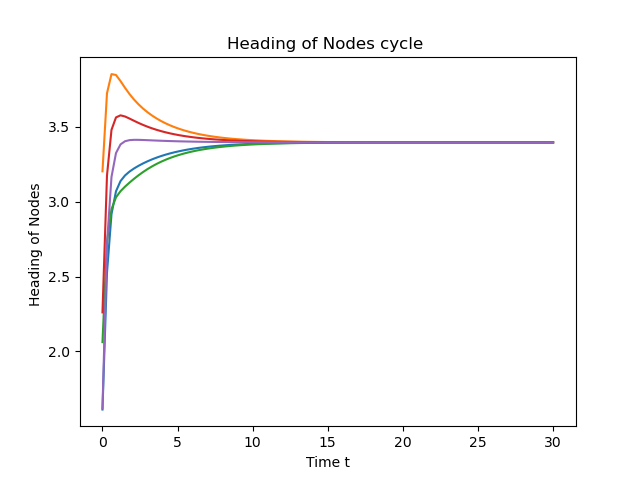
\includegraphics[width=\textwidth]{./img/p3_cycle1.png}
            \caption{Theta convergence of cycle graph }
        \end{subfigure}
        \begin{subfigure}{0.35\textwidth}
            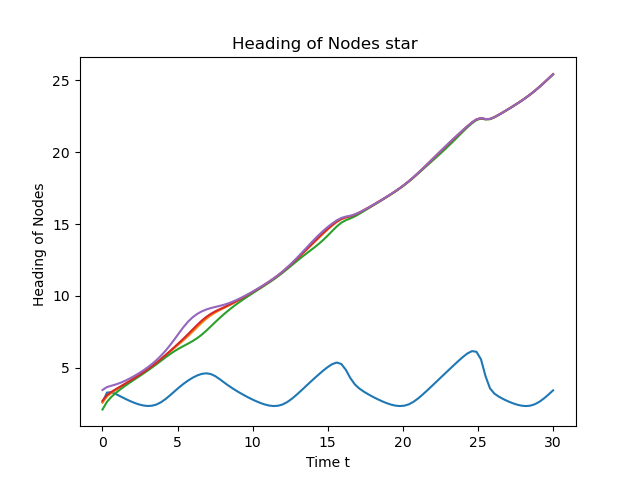
\includegraphics[width=\textwidth]{./img/p3_star1.png}
            \caption{Theta convergence of star graph }
        \end{subfigure}
        \begin{subfigure}{0.35\textwidth}
            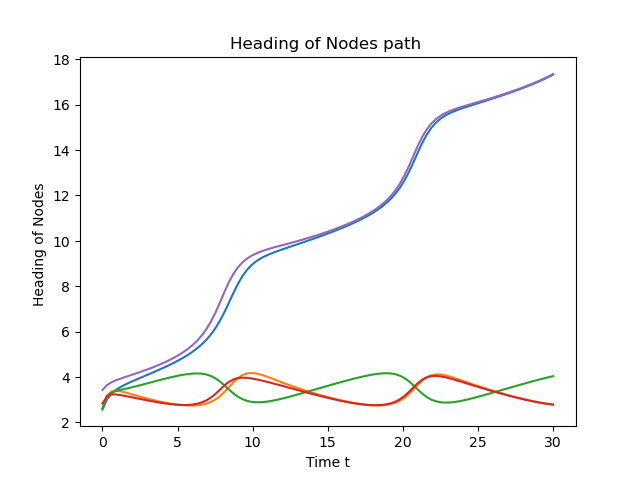
\includegraphics[width=\textwidth]{./img/p3_path1.png}
            \caption{Theta convergence of path graph }
        \end{subfigure}
        \begin{subfigure}{0.35\textwidth}
            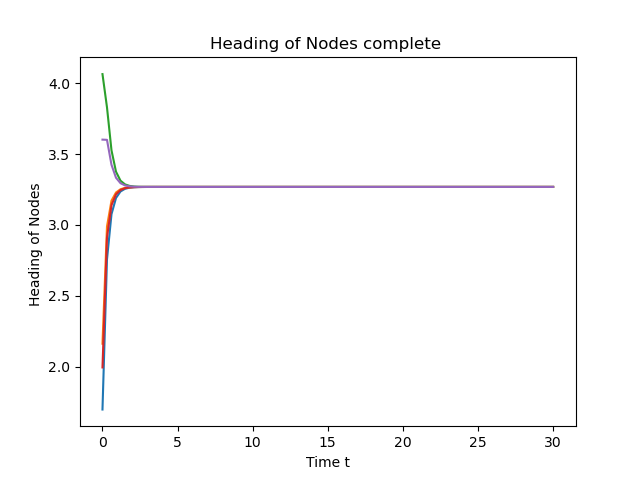
\includegraphics[width=\textwidth]{./img/p3_complete1.png}
            \caption{Theta convergence of complete graph }
        \end{subfigure}
    \end{figure*}
    \begin{figure*}[!h]
        \centering
        \begin{subfigure}{0.35\textwidth}
            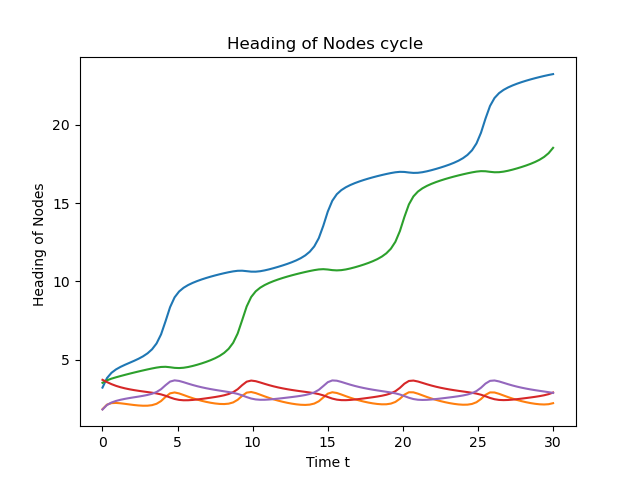
\includegraphics[width=\textwidth]{./img/p3_cycle2.png}
            \caption{Theta convergence of cycle graph }
        \end{subfigure}
        \begin{subfigure}{0.35\textwidth}
            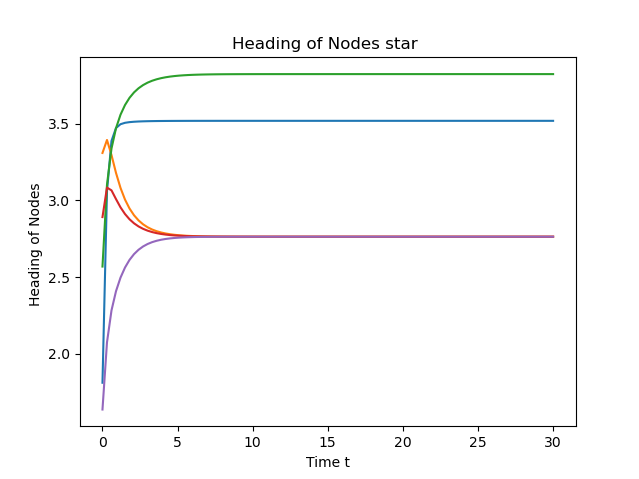
\includegraphics[width=\textwidth]{./img/p3_star2.png}
            \caption{Theta convergence of star graph }
        \end{subfigure}
        \begin{subfigure}{0.35\textwidth}
            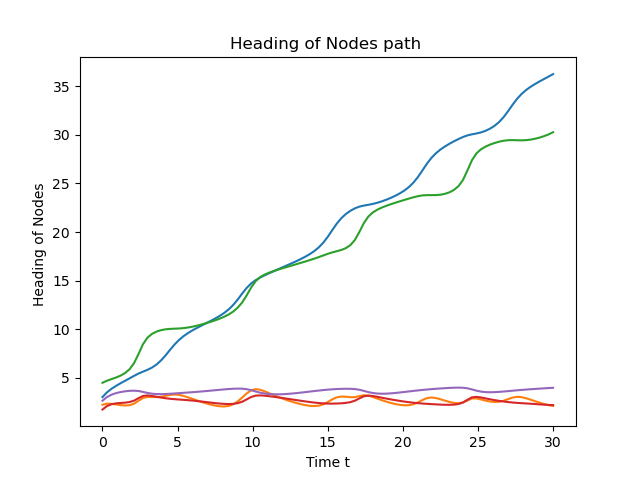
\includegraphics[width=\textwidth]{./img/p3_path2.png}
            \caption{Theta convergence of path graph }
        \end{subfigure}
        \begin{subfigure}{0.35\textwidth}
            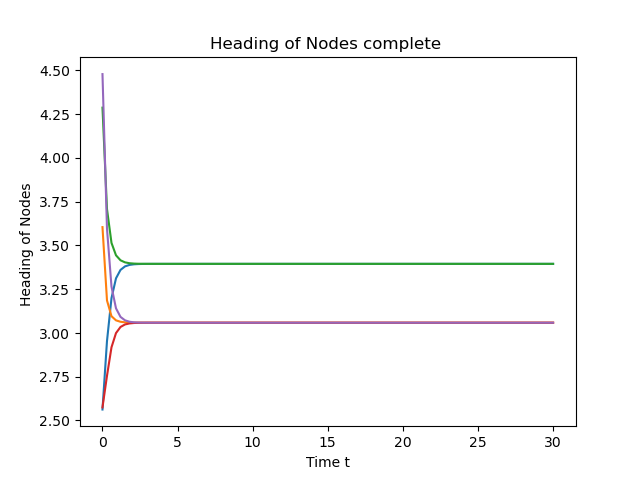
\includegraphics[width=\textwidth]{./img/p3_complete2.png}
            \caption{Theta convergence of complete graph }
        \end{subfigure}
    \end{figure*}
    Here we see that the cycle graph and copmlete graph again converges and star and path graph shows that some nodes are converging but oscillating and generally some nodes have same headings but keep increasing (meaning that they are changing speed of rotation but in same rate.) So with uniform angular velocity input, complete graph gurantees convergence. However, if there is discrepency in angular velocity inputs, then even the complete graph diverges. This is also obvious in intuitive way too. If one node was inputed with constant angular velocity, then those nodes would converge in a way that this constant angular velocity would cancel out. But if we input large enough different angular velocities to nodes, they would behave the same. Two nodes would oscillate and keep increasing their heading values, meaning the it is rotating anti closwise and their angular velosicty oscillating.  
    
    \begin{figure*}[!ht]
        \centering
        \begin{subfigure}{0.35\textwidth}
            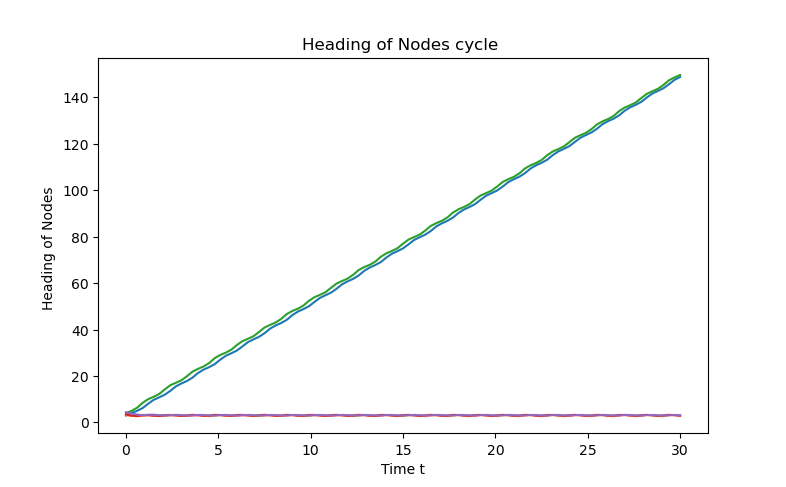
\includegraphics[width=\textwidth]{./img/p3_cycle3.png}
            \caption{Theta convergence of cycle graph }
        \end{subfigure}
        \begin{subfigure}{0.35\textwidth}
            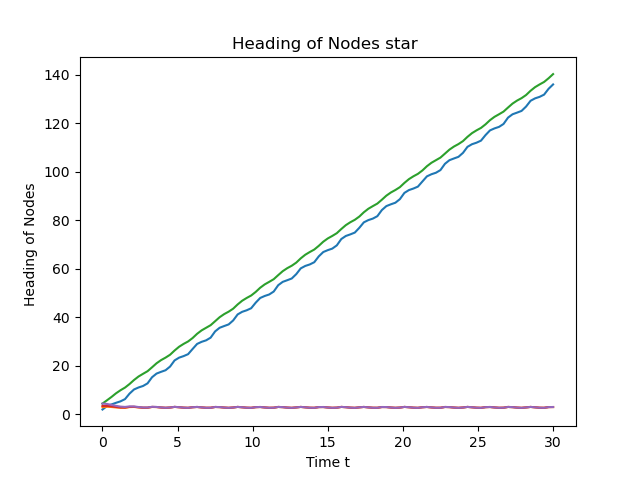
\includegraphics[width=\textwidth]{./img/p3_star3.png}
            \caption{Theta convergence of star graph }
        \end{subfigure}
        \begin{subfigure}{0.35\textwidth}
            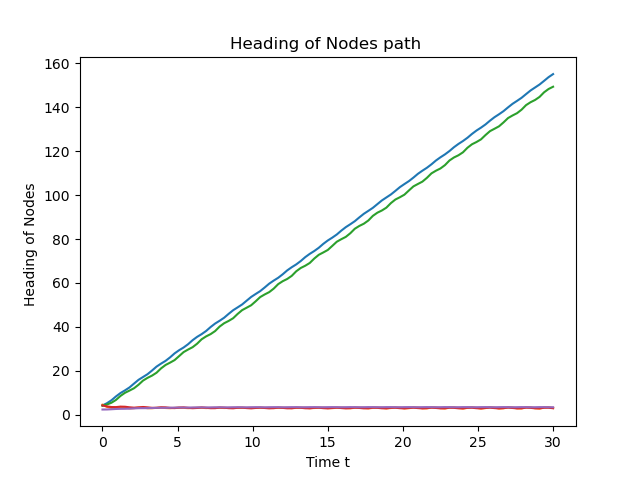
\includegraphics[width=\textwidth]{./img/p3_path3.png}
            \caption{Theta convergence of path graph }
        \end{subfigure}
        \begin{subfigure}{0.35\textwidth}
            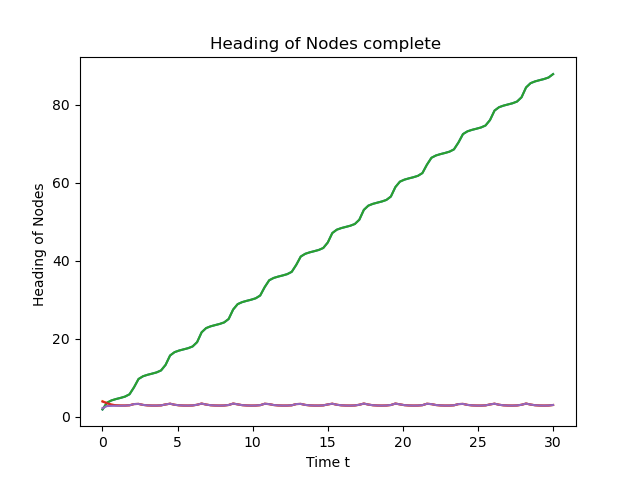
\includegraphics[width=\textwidth]{./img/p3_complete3.png}
            \caption{Theta convergence of complete graph }
        \end{subfigure}
    \end{figure*}
\end{problem}

\begin{problem}
    Provide an example for an agreement protocol on a digraph that always converges to the agreement subspace (from arbitrary initialization), yet does not admit a quadratic Lyapunov function of the form $\frac{1}{2} x^T x$, that testifies to its asymptotic stability with respect to the agreement subspace.

    If the agreement protocol is stochastic matrix, than it would not take in quadratic Lyapunov function, as we cannot integrate or take the derivative of stochastic data. Instead, we can use $V(z) = \max_i z_i - min_j z_j$ and $V(x(k+1)) - V(x(k)) < 0 $ to make sure that it is converging. We can discretize the agreement protocol by letting $z(k) = x(\delta x)$ for any $\delta \geq 0$. Then the agreement protocol can be expressed as such. 
    \begin{align*}
        z(k+1) = e^{-\delta L(D)}z(k)
    \end{align*}
    Since the stochasitc matrix $e^{-\delta L(D)}$ contatin one column of positive elements, (Corollary 4.2 in the textbook), the maximum and minimum states would decrease their differences if there is a difference in their states. Therefore quadratic form of Lyapunov function is not admitted in this case, but we can prove that $V(x(k+1)) - V(x(k)) < 0$ with the fact that the difference in minimum and maximum states are decreasing. Therefore this digraph would always converge to agreement subspace that corresponds to $V (z)= 0$, but not admitting quadratic form of Lyapunov function.

\end{problem}

\begin{problem}
Let $\lambda_1, \lambda_2, \lambda_3, \cdots, \lambda_n $ be the ordered eigenvalues of the graph Laplacian associated with an undirected graph. We have seen that the second eigenvalue $\lambda_2$ is important both as a measure of the robustness in the graph, and as a measure of how fast the protocol converges. Given that our job is to build up a communication network by incrementally adding new edges (communication channels) between nodes, it makes sense to try and make $\lambda_2$ as large as possible.
    
Write a program that iteratively adds edges to a graph (starting with a connected graph) in such a way that at each step, the edge (not necessarily unique) is added that maximizes $\lambda_2$ of the graph Laplacian associated with the new graph. In other words, implement the following algorithm: 

Step 0: Given G0 a spanning tree on n nodes. Set k=0

Step 1: Add a single edge to produce Gnew from Gk such that lambda2(Gnew) is maximized. Set k=k+1, Gk=Gnew

Repeat Step 1 until Gk=Kn for n = 10, 20, and 50. Did anything surprising happen?

\begin{minted}{python3}
def addEdge(G):
    start = G.nodes[0].copy()
    end = G.nodes[0].copy()
    max = 0    
    for node_i in G.nodes:
        G_temp = G.copy()
        for node_j in G.nodes:
            if node_i != node_j and ((node_i, node_j) not in G_temp.edges()):
                G_temp.add_edge(node_i, node_j)
                lambda2 = nx.laplacian_spectrum(G_temp)[1]
                if max < lambda2:
                    max = lambda2
                    start = node_i
                    end = node_j
    
    G.add_edge(start, end)
              
    return G
\end{minted}

First I created random graph with gnm random graph funtion. To make sure that I have the connected graph, I used $ \frac{(n-1)(n-2)}{2} $ for number of edges. Then iterated to add edges until the number of edges equal to number of edges in complete graph. 
\begin{figure*}[!ht]
    \centering
    \begin{subfigure}{0.35\textwidth}
        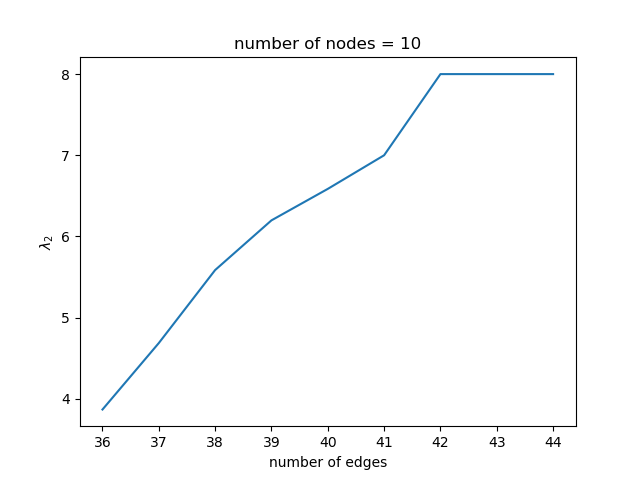
\includegraphics[width=\textwidth]{./img/p5_node10.png}
        \caption{n = 10 }
    \end{subfigure}
    \begin{subfigure}{0.35\textwidth}
        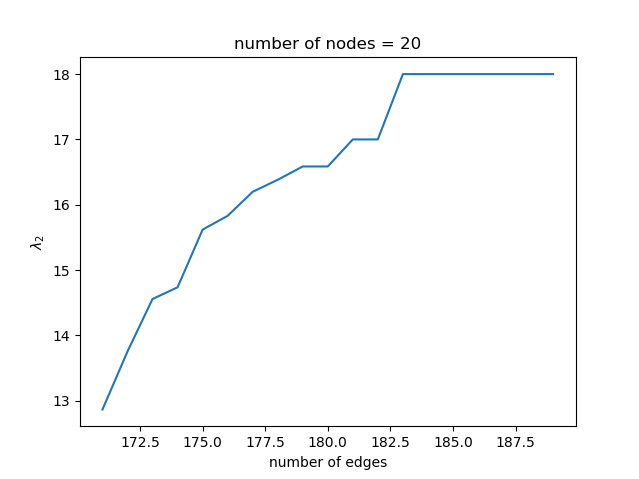
\includegraphics[width=\textwidth]{./img/p5_node20.png}
        \caption{n = 20 }
    \end{subfigure}
    \begin{subfigure}{0.35\textwidth}
        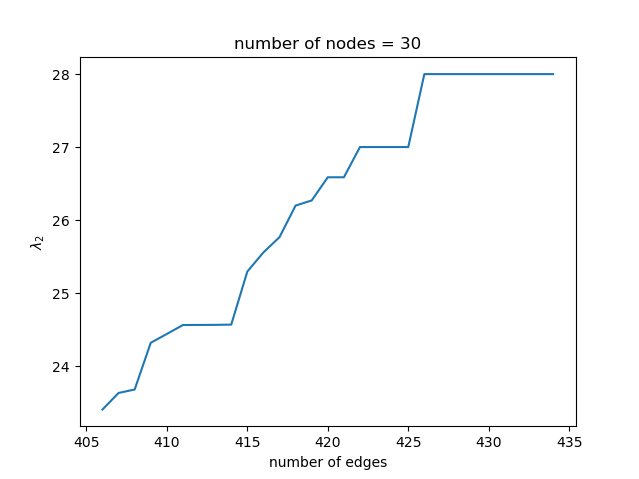
\includegraphics[width=\textwidth]{./img/p5_node30.png}
        \caption{n = 30}
    \end{subfigure}
    \begin{subfigure}{0.35\textwidth}
        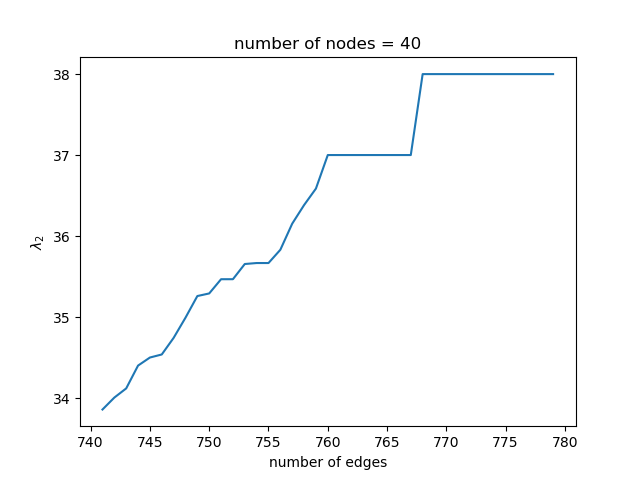
\includegraphics[width=\textwidth]{./img/p5_node40.png}
        \caption{n = 40 }
    \end{subfigure}
    
\end{figure*}
\newpage
\begin{figure*}[!h]
    \centering
    \begin{subfigure}{0.35\textwidth}
        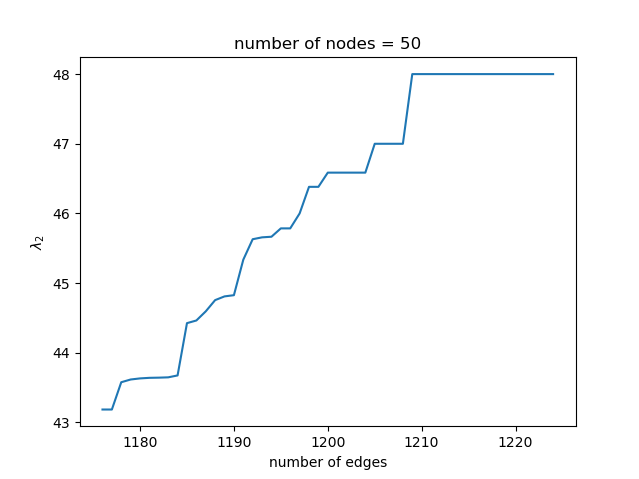
\includegraphics[width=\textwidth]{./img/p5_node50.png}
        \caption{n = 50}
    \end{subfigure}
    \begin{subfigure}{0.35\textwidth}
        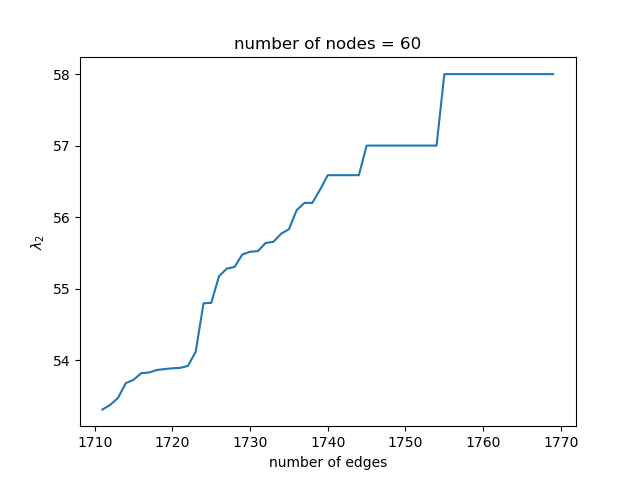
\includegraphics[width=\textwidth]{./img/p5_node60.png}
        \caption{n = 60 }
    \end{subfigure}
    \begin{subfigure}{0.35\textwidth}
        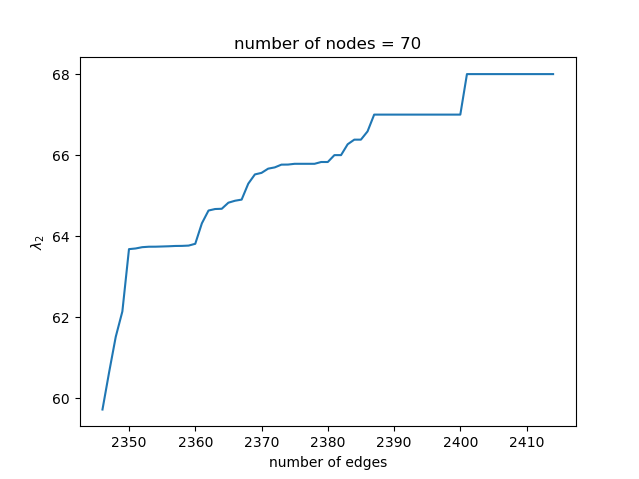
\includegraphics[width=\textwidth]{./img/p5_node70.png}
        \caption{n = 70 }
    \end{subfigure}
    \begin{subfigure}{0.35\textwidth}
        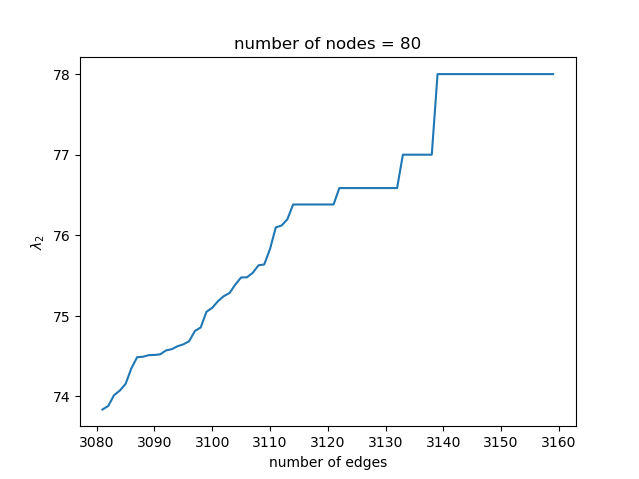
\includegraphics[width=\textwidth]{./img/p5_node80.png}
        \caption{n = 80 }
    \end{subfigure}

    \begin{subfigure}{0.35\textwidth}
        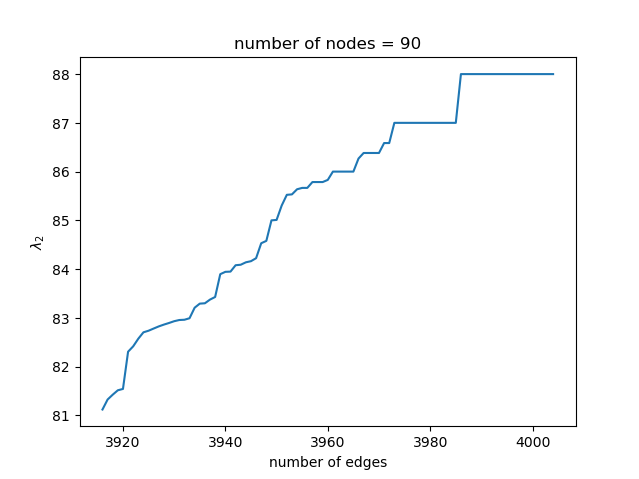
\includegraphics[width=\textwidth]{./img/p5_node90.png}
        \caption{n = 90 }
    \end{subfigure}
    \begin{subfigure}{0.35\textwidth}
        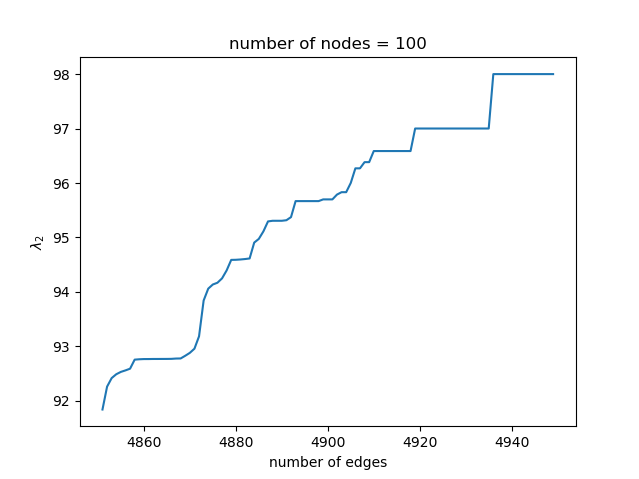
\includegraphics[width=\textwidth]{./img/p5_node100.png}
        \caption{n = 100 }
    \end{subfigure}
\end{figure*}


Clearly we see that the graphs are showing sudden jumps in connectivity or the lambda2. As I have incremented the number of edeges one by one, in some cases, lambda2 did not really change, but shows sudden increase in lambda2. 
\end{problem}
\newpage
\section*{Code problem 1}
\begin{minted}{python3}
import random
import networkx as nx
import matplotlib.pyplot as plt
import numpy as np
from scipy.integrate import odeint
from mpl_toolkits import mplot3d
def random_graphs_init(graph):
    for i in range(len(graph.nodes())):
        graph.nodes[i]['pos_x'] = random.randint(0, i + 100000)
        graph.nodes[i]['pos_y'] = random.randint(0, i + 100000)
        graph.nodes[i]['pos_z'] = random.randint(0, i + 100000)
        graph.nodes[i]['vel_x'] = random.randint(0, i + 100000)
        graph.nodes[i]['vel_y'] = random.randint(0, i + 100000)
        graph.nodes[i]['vel_z'] = random.randint(0, i + 100000)
        

    return graph

def get_input(x, G):
    k_p = 1
    k_v = 1
    u = np.zeros(len(x)//2)
    L_D = list(nx.directed_laplacian_matrix(G))
    for i in G.nodes():
        for j in G.neighbors(i):
            u[i] += -(k_p * L_D[i][j] * (x[j]- x[i] ) + k_v *L_D[i][j]* (x[len(x)//2 + j] - x[len(x)//2 + i] ))
    return u

def get_xdot(x, t, G):
    num = len(x)

    A = np.array([[0, 1], [0, 0]])
    B = np.array([0, 1])
    
    # Use Kronecker product to define the new dynamics
    Kronecker_A = np.kron(A, np.eye(num//2))
    
    u = get_input(x, G)

    dxdt = np.matmul(Kronecker_A, x) + np.kron(B, u)
    
    return dxdt 

def main():
    nums = [10]
    for num in nums:
        graphs = [nx.gnm_random_graph(num, 3 * num, directed=True)]
        for graph in graphs:
            graph = random_graphs_init(graph)
            t = np.linspace(0, 100, 1001)

            pos_vel_x = np.append(list(nx.get_node_attributes(graph, "pos_x").values()),list(nx.get_node_attributes(graph, "vel_x").values()) )
            pos_vel_y = np.append(list(nx.get_node_attributes(graph, "pos_y").values()),list(nx.get_node_attributes(graph, "vel_y").values()) )
            pos_vel_z = np.append(list(nx.get_node_attributes(graph, "pos_z").values()),list(nx.get_node_attributes(graph, "vel_z").values()) )
            
            
            trajectory_x = odeint(get_xdot, pos_vel_x, t, args=(graph,))
            trajectory_y = odeint(get_xdot, pos_vel_y, t, args=(graph,))
            trajectory_z = odeint(get_xdot, pos_vel_z, t, args=(graph,))

            plt.figure()
            plt.plot(t, trajectory_x[:,:num])
            plt.xlabel("Time t")
            plt.ylabel("Position x of Nodes ")
            plt.figure()
            plt.plot(t, trajectory_x[:,num:])
            plt.xlabel("Time t")
            plt.ylabel("Velocity x of Nodes ")
            plt.figure()
            plt.plot(t, trajectory_y[:,:num])
            plt.xlabel("Time t")
            plt.ylabel("Position y of Nodes ")
            plt.figure()
            plt.plot(t, trajectory_y[:,num:])
            plt.xlabel("Time t")
            plt.ylabel("Velocity y of Nodes ")
            plt.figure()
            plt.plot(t, trajectory_z[:,:num])
            plt.xlabel("Time t")
            plt.ylabel("Position z of Nodes ")
            plt.figure()
            plt.plot(t, trajectory_z[:,num:])
            plt.xlabel("Time t")
            plt.ylabel("Velocity z of Nodes ")
            plt.figure()
            ax = plt.axes(projection='3d')
            for i in range(num):
                ax.plot3D(trajectory_x[:,i], trajectory_y[:,i], trajectory_z[:,i])
                ax.scatter3D(trajectory_x[:,i], trajectory_y[:,i], trajectory_z[:,i])
            ax.set_xlabel("x")
            ax.set_ylabel("y")
            ax.set_zlabel("z")

    plt.show()

if __name__ == "__main__":
    main()
\end{minted}
\section*{Code problem 3}
\begin{minted}{python3}
import random
import networkx as nx
import matplotlib.pyplot as plt
import numpy as np
from scipy.integrate import odeint
from mpl_toolkits import mplot3d
def random_graphs_init(graph):
    for i in range(len(graph.nodes())):
        graph.nodes[i]['pos_x'] = random.randint(0, i + 100000)
        graph.nodes[i]['pos_y'] = random.randint(0, i + 100000)
        graph.nodes[i]['pos_z'] = random.randint(0, i + 100000)
        graph.nodes[i]['vel_x'] = random.randint(0, i + 100000)
        graph.nodes[i]['vel_y'] = random.randint(0, i + 100000)
        graph.nodes[i]['vel_z'] = random.randint(0, i + 100000)
        graph.nodes[i]['theta'] = random.uniform(np.pi/2, 3*np.pi/2)

    return graph

def get_xdot(theta, t, G, omega):
    D = nx.incidence_matrix(G).toarray()


    dxdt = omega + np.matmul(D,np.matmul(D.T, np.sin(theta)))
    
    return dxdt 

def main():
    nums = [5]
    for num in nums:
        names = ['cycle','path', 'star', 'complete']
        graphs = [nx.cycle_graph(num), nx.path_graph(num), nx.star_graph(num - 1), nx.complete_graph(num)]
        omega = [5, 0 ,5, 0, 0]
        k =0
        for graph in graphs:
            graph = random_graphs_init(graph)
            t = np.linspace(0, 30, 101)
            trajectory_theta = odeint(get_xdot, list(nx.get_node_attributes(graph, "theta").values()), t, args=(graph, omega))
            plt.figure()
            plt.plot(t, trajectory_theta)
            plt.xlabel("Time t")
            plt.ylabel("Heading of Nodes ")
            plt.title(f"Heading of Nodes {names[k]} ")
            k +=1
    plt.show()

if __name__ == "__main__":
    main()
\end{minted}
\section*{Code problem 5}
\begin{minted}{python3}
import random
import networkx as nx
import matplotlib.pyplot as plt
import numpy as np
from scipy.integrate import odeint
from mpl_toolkits import mplot3d

def addEdge(G):
    # diameter = nx.diameter(G)
    start = G.nodes[0].copy()
    end = G.nodes[0].copy()
    max = 0    
    for node_i in G.nodes:
        G_temp = G.copy()
        for node_j in G.nodes:
            if node_i != node_j and ((node_i, node_j) not in G_temp.edges()):
                G_temp.add_edge(node_i, node_j)
                lambda2 = nx.laplacian_spectrum(G_temp)[1]
                if max < lambda2:
                    max = lambda2
                    start = node_i
                    end = node_j
    
    G.add_edge(start, end)
                
    return G


def main():
    nums = [10, 20, 30, 40, 50, 60, 70, 80, 90, 100]
    for num in nums:
        graphs = [nx.gnm_random_graph(num,  (num-1)*(num-2)/2)]
        for graph in graphs:
            lambdas = []
            num_edges = []
            print(len(graph.edges()))
            while(len(graph.edges()) < num*(num-1)/2):
                lambdas.append(nx.laplacian_spectrum(graph)[1])
                num_edges.append(len(graph.edges()))
                graph = addEdge(graph)
                print(len(graph.edges()))
            plt.figure()
            plt.plot(num_edges, lambdas)
            plt.xlabel("number of edges")
            plt.ylabel("$\lambda_2$")
    plt.show()

if __name__ == "__main__":
    main()
\end{minted}
\end{document}